Un'analisi cruciale che può essere eseguita su un dataset di traiettorie è sicuramente la ricerca di oggetti che si muovono assieme.
Come detto nella \cref{subsec:fim-trajectory}, il mining di traiettorie pone l'attenzione sulla sul percorso e non sugli oggetti che ne fanno parte.
L'analisi dei gruppi di oggetti è molto simile nelle modalità a quella dei percorsi/luoghi frequenti, tuttavia le potenzialità informative sono totalmente diverse.
Analizzando i gruppi di oggetti si può vedere come questi variano nello spazio e nel tempo, ad esempio vedendo in quali gruppi un oggetto viaggia e per quanto.
Questa analisi può portare a diversi risultati, ad esempio sulla base di regolarità di certi gruppi di viaggio è possibile dedurre informazioni sulle modalità di viaggio di un utente.
Ancora la ricerca di gruppi di oggetti in movimento può fornire informazioni sul comportamento comune e quindi la natura di un certo gruppo: ad esempio un gruppo di molti utenti che viaggia insieme per un lungo periodo di tempo nel perimetro di una città potrebbe essere collegato a un tour turistico, al contrario un gruppo numeroso che viaggia assieme per un breve periodo potrebbe indicare un insieme di persone che stanno viaggiando su un mezzo pubblico.

Un \textit{co-movement} pattern~\cite{zheng2015trajectory} individua un gruppo di oggetti che si sono mossi assieme
per un certo tempo.
L'appartenenza a tale gruppo è determinata solitamente dalla vicinanza nello spazio.
La ricerca di questi pattern di movimento include diversi parametri che definiscono le caratteristiche dei gruppi individuati.
Varie tipologie di cluster sono state definite in letteratura sulla base dell'adozione e configurazione di questi parametri.

Prima di scendere nel dettaglio sui singoli pattern, occorre definire gli elementi principali del problema.
Innanzitutto dato un dataset di traiettorie \(TR_{db} = \{tr_{1}, \ldots, tr_{n}\} \), da questo viene derivato il dataset
degli oggetti che hanno generato quelle traiettorie, \(O_{db} = \{ o_{1}, \ldots, o_{m} \}, m \leq n\)
e un dataset contenente tutti i possibili istanti temporali del primo dataset
\(T_{db} = \{t_{1}, \ldots, t_{k}\} \).
In generale, nella ricerca di co-movement pattern si ricerca un gruppo di oggetti \(O = \{ o_{1}, \ldots, o_{p} \}, O \subseteq O_{db} \)
tale che il corrispondente \(T = \{t_{1}, \ldots, t_{j}\} T \subseteq T_{sb}\), definito come l'insieme degli istanti in cui gli oggetti di \(O\) sono vicini, goda di certe proprietà, come
ad esempio una lunghezza minima, oppure una continuità all'interno del tempo.
Due parametri comuni a tutti i pattern di movimento sono \(m\), che individua una
soglia minima per la dimensione di \(O\) e \(k\), limite inferiore al numero
di istanti temporali in cui il gruppo in questione è considerato vicino.
La \cref{tab:co-movement-pattern} riassume i principali vincoli che saranno adoperati nella ricerca di pattern.

\begin{table}[H]
    \centering
   \begin{tabular}{||c c||}
 \hline
     Parametro & Vincolo espresso\\ [0.4ex] 
 \hline\hline
     \(m\) & dimensione minima del gruppo \\ 
 \hline
    \(k\) & minimo numero di istanti temporali in cui il gruppo è stato assieme \\ 
 \hline
     \(l\) & lunghezza minima di ogni sotto-sequenza continua di \(T\)\\ 
 \hline
\end{tabular}
    \caption{Parametri per la ricerca di pattern di co-movimento e il loro significato}
    \label{tab:co-movement-pattern}
\end{table}

I pattern di movimento possono essere suddivisi in due categorie a seconda dell'algoritmo di clustering utilizzato per riconoscere quali punti siano vicini e quali no.
Se viene impiegato un clustering basato sulla distanza, allora si parla di \textit{distance based pattern} (pattern basati sulla distanza), mentre se viene utilizzato un algoritmo basato sulla densità, allora si parla di \textit{density based pattern}.
Per semplicità nelle tipologie di pattern presentate d'ora in poi si fa riferimento a pattern basati sulla densità.

Il primo pattern di movimento individuabile alla luce dei vincoli è \textit{swarm}~\cite{li2010swarm}.
In maniera informale, swarm ricerca gruppi di \(m\) oggetti che hanno viaggiato assieme per almeno \(k\) istanti temporali senza porre alcun ulteriore vincolo.
Uno swarm può essere definito come segue:

\begin{definition}[Swarm]\label{definition:swarm}

  Una coppia \( \{ O, T \} \) si definisce swarm se:

  \begin{center}

    \(
      \begin{cases}
         \forall t \in T,\exists c \; t.c \; O \in c \\
         |O| \geq m \\
         |T| \geq k

      \end{cases}
      \)

  \end{center}
\end{definition}

La~\cref{definition:swarm} formalizza i seguenti vincoli:
ad ogni istante di \(T\) gli oggetti di \(O\) devono appartenere a uno stesso cluster,
il gruppo deve essere poi rilevante dal punto di vista degli elementi (\(m\)) e del tempo trascorso
(\(k\)).
Per quanto riguarda il primo vincolo, è possibile utilizzare varie metriche per fare clustering
sulla dimensione spaziale del dataset, tuttavia l'algoritmo più utilizzato per la ricerca di swarm
è DBSCAN (\cref{sec:clustering}).


Il concetto di swarm può essere ulteriormente raffinato in quello di \textit{closed swarm}:
un closed swarm intuitivamente si definisce allo stesso modo di uno swarm, ma con l'ulteriore
vincolo di considerare la massima sequenza di istanti in cui gli oggetti dentro \(O\) risultano vicini
tra di loro (chiusura rispetto al tempo) oppure il numero massimo di oggetti dato un certo \(T\) (chiusura rispetto agli oggetti).
Formalmente, ciò è espresso nella~\cref{definition:closed-swarm}

\begin{definition}[Closed Swarm]\label{definition:closed-swarm}

  Una coppia \( \{ O, T \} \) si definisce closed swarm se:

  \begin{center}

    \(
      \begin{cases}
         \{ O, T \} \; risulta \; swarm   \\
         \nexists O' \; t.c. \;  \{ O \cup O', T \} risulta \; swarm   \\
         \nexists T' \; t.c. \;  \{ O, T \cup T' \} risulta \; swarm
      \end{cases}
    \)

  \end{center}

\end{definition}

Com'è possibile vedere in~\cref{fig:chap-1:SwarmExample} (Fonte:~\cite{phan2016all}), la ricerca di swarm produce riconosce
il gruppo \( \{ o_{1}, o_{2}\} \) in quanto i due oggetti risultano avere viaggiato vicini per almeno
tre istanti temporali (\(t_{1}, t_{3}, t_{4}\)).

\begin{figure}
  \centering
  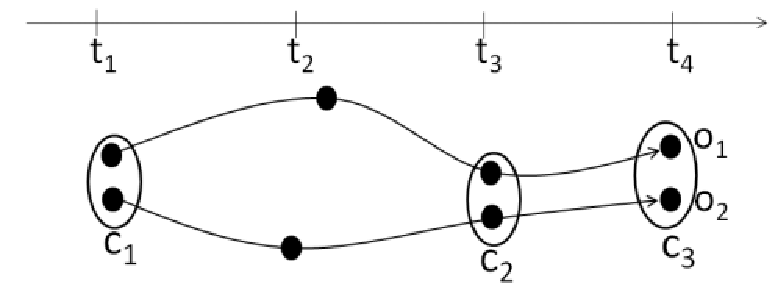
\includegraphics[width=\textwidth]{/sec-2/SwarmExample.pdf}
  \caption{Ricerca di swarm su un dataset fissati \(m=2\) e \(k=3\), Fonte:\cite{DBLP:journals/ijitdm/PhanPT16}}%
  \label{fig:chap-1:SwarmExample}
\end{figure}


Entrambi i pattern appena presentati rilassano al massimo i vincoli sul tempo,
accettando gruppi aventi istanti temporali parecchio distanti gli uni dagli altri.
Un tipo di analisi che aggiunge un rigido vincolo sulla continuità degli istanti temporali è
la ricerca di \textit{convoy}~\cite{jeung2008convoy}: un convoy per definizione è un raggruppamento di oggetti \(O\) in cui
tutti gli istanti in \(T\) sono consecutivi, mantenendo i precedenti vincoli sulle dimensioni del
gruppo e sul tempo trascorso assieme.

\begin{definition}[Convoy]\label{definition:convoy}
  Una coppia \( \{ O, T \} \) si definisce convoy se:
  \begin{center}
    \(
      \begin{cases}
         \{ O, T \} \; risulta \; swarm   \\
      \forall t_{i} \in T, t_{i+1} = t_{i} + 1
      \end{cases}
    \)

  \end{center}
\end{definition}

Convoy utilizza un algoritmo basato su densità, come ad esempio DBSCAN, per determinare
la vicinanza o meno di due oggetti in base all'appartenenza a un certo cluster ad ogni
\(t_{i}\).
Qualora si voglia adottare un algoritmo basato sulla distanza per determinare la vicinanza, allora i
pattern individuati sono chiamati \textit{flock}~\cite{benkert2008reporting} pattern.
La~\cref{fig:chap-1:ConvoyExample} (Fonte:~\cite{phan2016all}) mostra un esempio di ricerca di convoy: fissati \(m=2\)
e \(k=3\), risulta come pattern valido \( \{ o_{1}, o_{2}\} \),
\( \{ o_{1}, o_{2}, o_{3}\} \) viene scartato in quanto non soddisfa il vincolo di continuità
sugli istanti temporali.

\begin{figure}
  \centering
  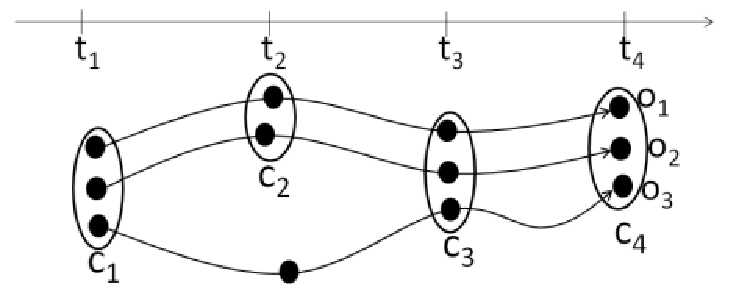
\includegraphics[width=\textwidth]{/sec-2/ConvoyExample.pdf}
  \caption{Ricerca di convoy su un dataset fissati \(m=2\) e \(k=3\), Fonte:\cite{DBLP:journals/ijitdm/PhanPT16}}%
  \label{fig:chap-1:ConvoyExample}
\end{figure}

Convoy e swarm rappresentano i due casi limite per quanto riguarda la rigidità dei vincoli temporali:
swarm rilassa totalmente la continuità mentre convoy esige una rigidità assoluta nella sequenza
degli istanti temporali.
Una via di mezzo tra i due estremi è individuata nel pattern \textit{group}~\cite{wang2006efficient}.
Un pattern group individua un insieme di convoy disgiunti nel tempo relativi allo stesso gruppo di oggetti \(O\);
interpretando ogni convoy come un singolo punto temporale \(t_{s}\), un pattern group può essere visto come uno swarm
di convoy.
Ognuno dei singoli punti così individuati dovrà risultare come valido convoy, si definisce
il parametro \textit{l} come la lunghezza di istanti condivisi in ognuno dei punti individuati.
Il valore di \(k\) per lo swarm così individuato indica il numero minimo di convoy necessari per il riconoscimento di group,
solitamente tale valore è fissato a \(1\).

\begin{definition}[Group]\label{definition:group}
  Definito \(T\) come l'insieme totale di istanti in cui gli oggetti di \(O\) sono vicini,
  \(T_s\) come l'insieme delle sotto-sequenze continue e disgiunte \(T' \subseteq T\)
  una coppia \( \{ O, T_{s} \} \) si definisce group se:
  \begin{center}
    \(
      \begin{cases}
         \{ O, T_{s} \} \; risulta \; swarm   \\
      \forall t_{s} \in T_{s}, \; |t_{s}| \geq l
      \end{cases}
    \)

  \end{center}
\end{definition}

\begin{figure}
  \centering
  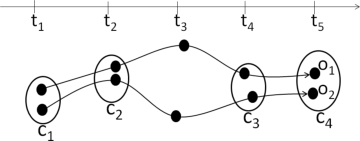
\includegraphics[width=\textwidth]{res/fig/sec-2/Group.pdf}
  \caption{Ricerca di group su un dataset fissati \(m=2\) e \(l=2\), Fonte:\cite{DBLP:journals/ijitdm/PhanPT16}}%
  \label{fig:chap-1:GroupExample}
\end{figure}

La \cref{fig:chap-1:GroupExample} contiene un esempio di ricerca di pattern group, com'è possibile vedere il parametro \(k\) non è considerato nella ricerca.

Group introduce la possibilità di ricercare gruppi con una continuità rilassata, tuttavia
non pone nessun vincolo sul numero complessivo di istanti necessari per considerare un pattern interessante.
Per integrare questo parametro, è stato definito il pattern \textit{platoon}~\cite{li2015efficient}.
Questo approccio interpreta diversamente il valore di \textit{k} rispetto a quanto fatto in
group: se in quest'ultimo approccio \(k\) indicava il numero di convoy necessari per individuare
un raggruppamento valido, ora \(k\) indica il numero di istanti assoluti necessari per
un gruppo valido.
In termini formali, il pattern platoon può essere definito come segue:

\begin{definition}[Platoon]\label{definition:platoon}
  Definito \(T\) come l'insieme totale di istanti in cui gli oggetti di \(O\) sono vicini,
  \(T_s\) come l'insieme delle sotto-sequenze continue e disgiunte \(T' \subseteq T\)
  una coppia \( \{ O, T \} \) si definisce platoon se:
  \begin{center}
    \(
      \begin{cases}
         \{ O, T \} \; risulta \; swarm   \\
      \forall T' \in T_{s}, \; |T'| \geq l
      \end{cases}
    \)
  \end{center}
\end{definition}

\begin{figure}
  \centering
  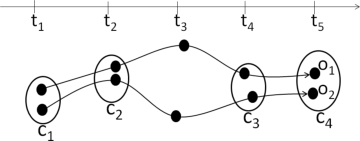
\includegraphics[width=\textwidth]{res/fig/sec-2/Group.pdf}
  \caption{Ricerca di Platoon con \(m = 2\), \(k = 3\), \(l=2\), Fonte:\cite{DBLP:journals/ijitdm/PhanPT16}}%
  \label{fig:chap-1:PlatoonExample}
\end{figure}

Com'è possibile vedere nella \cref{fig:chap-1:PlatoonExample}, in questo caso i risultati di platoon e group coincidono.
Tuttavia non è sempre così: confrontando l'applicazione dei pattern appena descritti a uno stesso dataset, la 
\cref{fig:chap-1:AllExample} mostra
quali sono le differenze, a parità di valori di \(m, k \) e \(l\), tra i diversi pattern di movimento.
Dalla figura in questione emergono chiaramente le differenze tra i gruppi individuati dai
vari pattern: ad esempio group riconosce \( \{ o_{3}, o_{4}, o_{5}\} \) negli istanti \( \{ 1, 2 \} \)
poiché la lunghezza di tale sotto-sequenza risulta uguale ad \(l\); platoon invece spezza
il raggruppamento in \( \{ o_{3}, o_{4} \}, \{ o_{4}, o_{5} \} \) poiché quest'ultimo non
avrebbe rispettato il vincolo sulla lunghezza minima degli istanti \(k\).
Convoy e Swarm invece riconoscono i pattern aventi una continuità assoluta in un caso,
totalmente assente nell'altro.
Entrambi ignorano il valore del parametro \(l\).

\begin{figure}
  \centering
  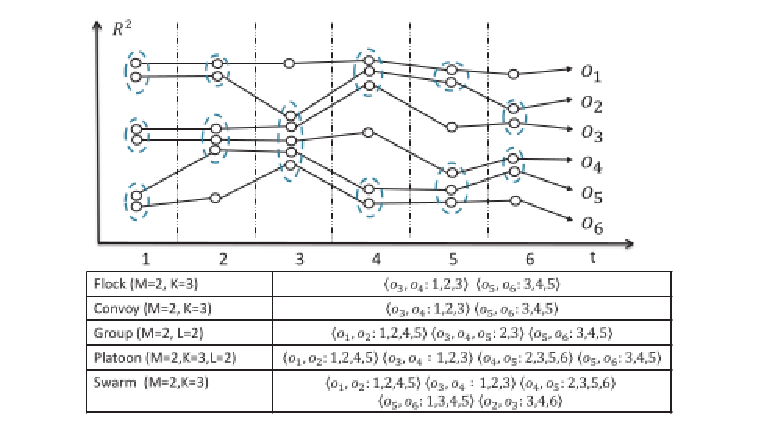
\includegraphics[width=\textwidth]{/sec-2/AllExamples.pdf}
  \caption{Ricerca dei principali pattern di movimento su un dataset fissati \(m=2\), \(k=3\) e \(l=2\), Fonte:~\cite{DBLP:journals/pvldb/FanZWT16}}%
  \label{fig:chap-1:AllExample}
\end{figure}

La \cref{tab:co-movement-pattern-list} riassume i pattern di co-movimento appena presentati in relazione ai vincoli espressi.

\begin{table}[H]
    \centering
   \begin{tabular}{||c c c c||}
 \hline
     Pattern & Dimensione del gruppo & Numero di istanti & Continuità \\ [0.4ex] 
 \hline\hline
     swarm & \(m\) & \(k\) & - \\ 
 \hline
    closed swarm & \(m\) & \(k\) & - \\ 
 \hline
     convoy & \(m\) & \(k\) & globale \\ 
  \hline
     group & \(m\) & - & locale \\
  \hline
    platoon & \(m\) & \(k\) & locale \\ 
 \hline
\end{tabular}
    \caption{Parametri per la ricerca di pattern di co-movimento e il loro significato}
    \label{tab:co-movement-pattern-list}
\end{table}
